\documentclass[tikz]{standalone}
\usepackage{tikz}

\begin{document}

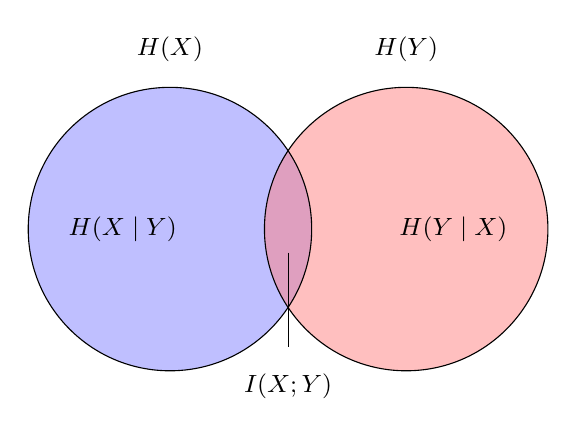
\begin{tikzpicture}[every node/.style={font=\small}]
    % 圆半径
    \def\r{1.8}

    % 圆心位置
    \coordinate (Xc) at (0,0);
    \coordinate (Yc) at (3,0);

    % 着色：左 H(X)，右 H(Y)，交叠区域颜色更深
    \fill[blue!50,opacity=0.5] (Xc) circle (\r);
    \fill[red!50,opacity=0.5]  (Yc) circle (\r);

    % 边界
    \draw (Xc) circle (\r);
    \draw (Yc) circle (\r);

    % 顶部标 H(X), H(Y)
    \node[above] at (0, \r+0.2) {$H(X)$};
    \node[above] at (3, \r+0.2) {$H(Y)$};

    % 条件熵部分：左右各一块
    \node at (-0.6,0) {$H(X\mid Y)$};
    \node at (3.6,0) {$H(Y\mid X)$};

    % 中间交叠部分：互信息
    \draw (1.5,-0.3)--(1.5,-1.5);
    \node at (1.5,-2) {$I(X;Y)$};

\end{tikzpicture}

\end{document}